\subsection{Conditional GANs}
\begin{frame}{}
    \LARGE GAN Variant: \\[1.5ex] \textbf{Conditional GANs}
\end{frame}

\begin{frame}[allowframebreaks]{Conditional GAN}
\begin{itemize}
    \item In addition to random noise, a condition is added to the generator input. 
    \item The discriminator also receives this condition.
\end{itemize}
\begin{figure}
    \centering
    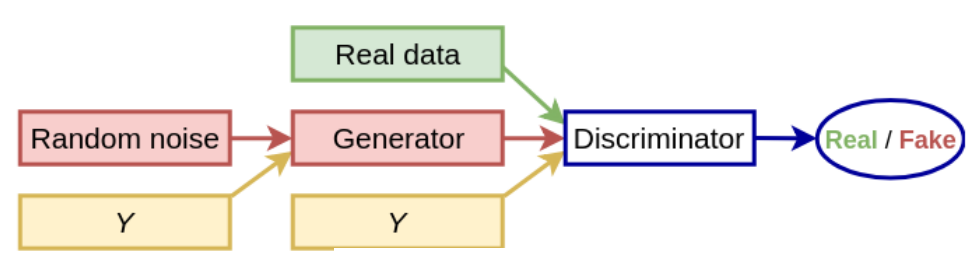
\includegraphics[height=0.8\textheight, width=\textwidth, keepaspectratio]{images/gan/cond_gan_1.png}
\end{figure}

\framebreak
\begin{itemize}
    \item Discriminator Loss:
    \begin{align*}
    \mathcal{L}^{(D)} \left( \theta^{(G)}, \theta^{(D)} \right) =\ & 
    - \mathbb{E}_{x \sim p_{data}} \left[ \log D(x|y) \right] \\
    & - \mathbb{E}_{z \sim p_z(z),\ y \sim p_{data}(y)} \left[ \log(1 - D(G(z|y))) \right]
    \end{align*}
    \item Generator Loss:
    $$
    \mathcal{L}^{(G)} \left( \theta^{(G)}, \theta^{(D)} \right) = - \mathbb{E}_z \left[ \log D(G(z|y)) \right]
    $$
\end{itemize}

\framebreak
\begin{figure}
    \centering
    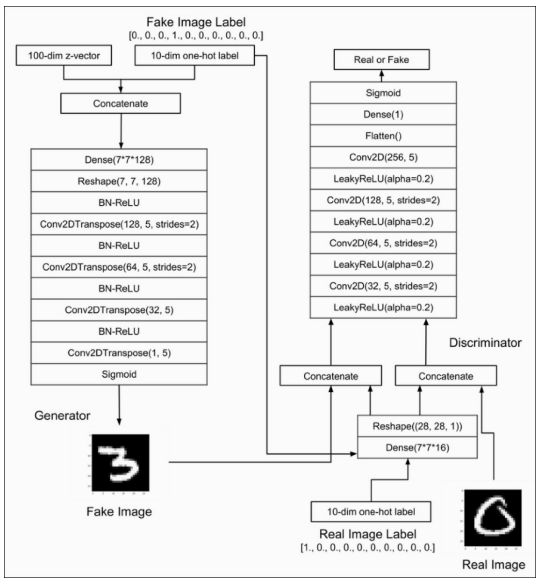
\includegraphics[height=0.8\textheight, width=\textwidth, keepaspectratio]{images/gan/cond_gan_2.png}
    \caption*{A conditional GAN architecture for the MNIST digits dataset.}
\end{figure}

\end{frame}

\begin{frame}[allowframebreaks]{Condional GAN - Image to Image}

\begin{figure}
    \centering
    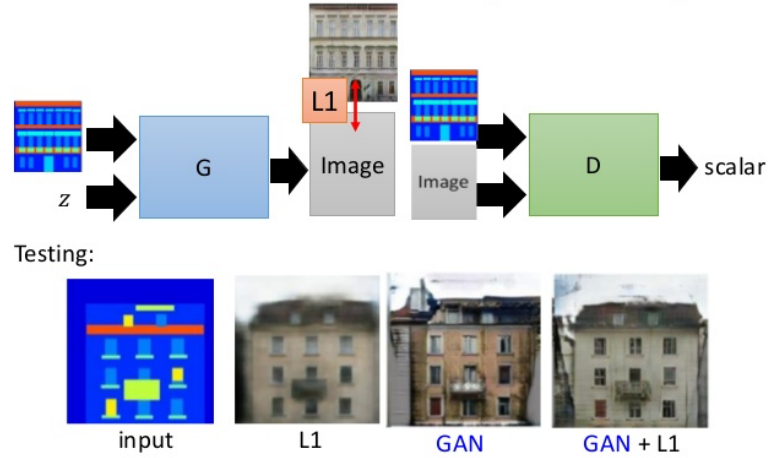
\includegraphics[height=0.75\textheight, width=\textwidth, keepaspectratio]{images/gan/cond_gan_3.png}
    \caption*{Using L1 loss in addition in GAN loss can help in image to image translation}
\end{figure}

\framebreak

\begin{figure}
    \centering
    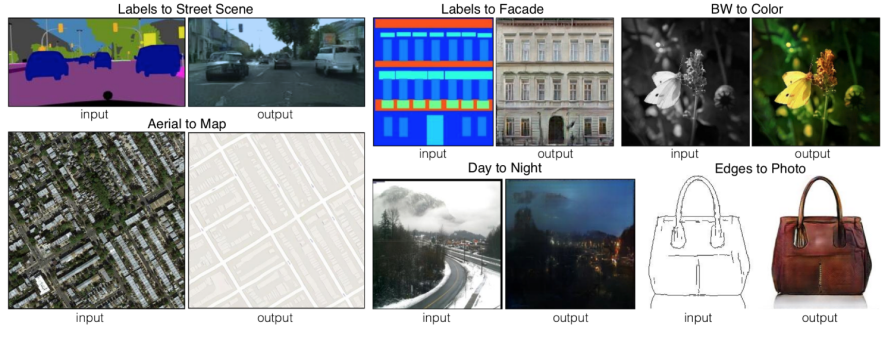
\includegraphics[height=0.8\textheight, width=\textwidth, keepaspectratio]{images/gan/cond_gan_4.png}
    \caption*{Image to Image translation with condional GANs}
\end{figure}
    
\end{frame}